%!TEX root = ../problems.tex
% \begin{figure}[h!]
%   \vspace{-20pt}
%   \begin{center}
%     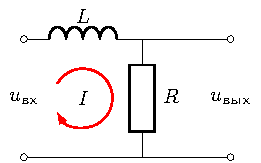
\includegraphics[scale=1.5]{chem/task2}
%   \end{center}
%   \vspace{-20pt}
%   \caption{$RL$--контур}
%   \vspace{-10pt}
% \end{figure}

\begin{figure}[h!]
\centering
\begin{minipage}{0.4\textwidth}
\centering
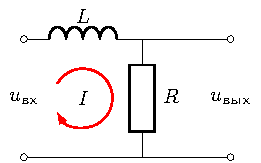
\includegraphics[width=\linewidth]{chem/task2}
\caption{$RL$--контур}
\label{fig:2figsA}
\end{minipage}
\qquad
\begin{minipage}{0.4\textwidth}
\centering
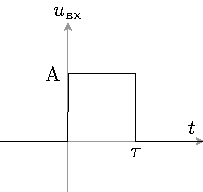
\includegraphics[width=\linewidth]{ris/task2_input}
\caption{Входное напряжение}
\label{fig:2figsB}
\end{minipage}
\end{figure}

\begin{task}
Определить отклик выхода RL-цепи, изображенной на рисунке, на воздействие прямоугольного импульса длительностью $\tau_0$. Нарисовать график $u_\out\qty(t)$. При выполнении какого условия будет осуществляться приближенное интегрирование входной цепи? 
\end{task}

\begin{proof}[\rm{\textbf{Решение}}]
Эквивалентная схема (картиночка)
 \begin{equation}
	u_\in\qty(t)\risingdotseq \frac{A}{p}-\frac{A}{p}\cdot e^{-p\tau}=\frac{A}{p}\qty(1-e^{-p\tau})
\end{equation}
По второму правилу Кирхгофа, сумма падений напряжения на всех элементах цепи равна ЭДС. В нашем случае возможное начальное напряжение на катушке мы относим к ЭДС, а сумму падений напряжения записываем как ток в контуре на суммарный импеданс контура:
\begin{equation}
	\eds=Z(p)\cdot I(p) \quad \Rightarrow \quad
	\frac{A}{p} \qty(1-e^{-p\tau}) + i_L\qty(0)L=\qty(pL+R)I\qty(p)
\end{equation}
Отсюда выражаем ток в контуре:
\begin{equation}
	I\qty(p)=\frac{\frac{A}{p}\qty(1-e^{-p\tau})}{pL+R} + 
		\frac{i_L\qty(0)L}{pL+R}
\end{equation}
% С другой стороны, $u_\in=u_R+u_L$, и отсюда
% \begin{gather}
% \frac{A}{p}\qty(1-e^{-p\tau})=
% 	I\qty(p)R+u_L\qty(p) \Rightarrow \\
% %
% u_L\qty(p) = 
% 	\frac{A}{p}\qty(1-e^{-p\tau})-I\qty(p)R =
% 	\frac{A}{p}\qty(1-e^{-p\tau}) - 
% 		\frac{\frac{AR}{p}\qty(1-e^{-p\tau})}{pL+R} - 
% 		\frac{i_L\qty(0)LR}{pL+R} = \\ =
% %
% \frac{A}{p}\qty(1-e^{-p\tau}) - 
% 	\frac{A\frac{R}{L}}{p\qty(p+\frac{R}{L})} + 
% 	\frac{A\frac{R}{L}}{p\qty(p+\frac{R}{L})}e^{-p\tau} - 
% 	\frac{i_L\qty(0)R}{p+\frac{R}{L}} \LT \\ \LT
% %  
% \cancel{A\H\qty(t)}-
% 	\cancel{A\H\qty({t}-\tau)}-
% 	A\qty(\cancel{1}-e^{-\frac{Rt}{L}}) \H\qty(t) +
% 	A\qty(\cancel{1}-e^{-\frac{R}{L}\qty(t-\tau)}) \H\qty(t-\tau) - 
% 	i_L\qty(0)Re^{\frac{-R}{L}t} \H\qty(t) = \\=
% %
% Ae^{-\frac{Rt}{L}}\cdot \H\qty(t)-
% 	Ae^{-\frac{R\qty(t-\tau)}{L}}\cdot \H\qty(t-\tau)-
% 	i_L\qty(0)Re^{-\frac{Rt}{L}}\cdot \H\qty(t)
% \end{gather}
% Отсюда получаем окончательно выражение для напряжения на индуктивности:
% \begin{equation}
% u_L\qty(t)=
% \qty(A-i_L\qty(0)R)e^{-\frac{Rt}{L}}\cdot \H\qty(t) - 
% 	Ae^{-\frac{R\qty(t-\tau)}{L}}\cdot \H\qty(t-\tau)
% \end{equation}
% Нам надо
Теперь мы можем найти и выходное напряжение -- напряжение на резисторе:
\begin{gather}
	u_\out (p) \equiv u_R\qty(p)=I\qty(p)R=
		\frac{AR\qty(1-e^{-p\tau})}{p\qty(pL+R)}+
		\frac{i_L\qty(0)RL}{pL+R}=
	\frac{\frac{AR}{L}\qty(1-e^{-p\tau})}{p\qty(p+\frac{R}{L})}+
		\frac{i_L\qty(0)R}{p+\frac{R}{L}} 
		=\\=
	A\frac{\frac{R}{L}}{p\qty(p+\frac{R}{L})}-
		A\frac{\frac{R}{L}}{p\qty(p+\frac{R}{L})}e^{-p\tau}+
		i_L\qty(0)R\frac{1}{p+\frac{R}{L}} 
		% \LT \\ \LT 
	% A\qty(1-e^{-\frac{Rt}{L}})\cdot \H\qty(t)-
		% A\qty(1-e^{-\frac{R\qty(t-\tau)}{L}})\cdot \H\qty(t-\tau)+
		% i_L\qty(0)Re^{-\frac{Rt}{L}}\cdot \H\qty(t)
\end{gather}
Используя свойства преобразования Лапласа
\begin{gather}
	\frac{\alpha}{p(p+\alpha)}\LT (1-e^{-\alpha t})\H(t)\\
	\frac{1}{(p+\alpha)}\LT e^{-\alpha t}\H(t)\\
	e^{{-p\tau}}F(p) \LT f(t-\tau)\H(t-\tau), \qq{где} F(p) \LT f(t)
\end{gather}
Из выражения $u_\out(p)$ элементарно получаем оригинал $u_\out(t)$:
\begin{equation}
	u_\out(t)=A\qty(1-e^{-\frac{Rt}{L}})\cdot \H\qty(t)-
		A\qty(1-e^{-\frac{R\qty(t-\tau)}{L}})\cdot \H\qty(t-\tau)+
		i_L\qty(0)Re^{-\frac{Rt}{L}}\cdot \H\qty(t)
\end{equation}
\begin{figure}[h!]
	\centering
	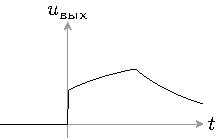
\includegraphics[width=0.4\textwidth]{ris/task2_out.pdf}	
	\caption{$u_\out(t)$}
	% \label{fig:figure1}
\end{figure}
График построен при $i_L(0)R=\frac{A}{2}$.  

\paragraph{Условие интегрирования.} 
Рассмотрим очевидное равенство $u_\in=u_L+u_\out$.
Перепишем это выражение:
\begin{equation}
	u_\in=L\dv{I}{t}+\underbrace{IR}_{u_\out}
\end{equation}
Проинтегрируем его по времени:
\begin{equation}
	\int u_\in \dd{t}=
		\frac{L}{R}\underbrace{IR}_{u_\out}+R\int I \dd{t}
\end{equation}
Если будет выполнено условие
\begin{equation}
	\label{eq:int}
	% \abs{L\dv{u_L}{t}} \ll \abs{\frac{R}{L} u_L} \qquad
	\abs{R\int I \dd{t}} \ll \abs{LI} \quad \Rightarrow \quad
	\abs{\int I \dd{t}} \ll \abs{\frac{L}{R}I}
\end{equation}
То выходное напряжение с точностью до множителя интегрирует входное:
\begin{equation}
	u_\out=\frac{1}{\tau_\text{цепи}}\int u_\in \dd{t}
\end{equation}
где $\tau_\text{цепи}=\frac{L}{R}$.

Выясним смысл неравенства модулей на примере гармонических сигналов. Пусть входное напряжение гармоническое $u_\in=u_0e^{j\omega t}$. Тогда ток в контуре: $I=I_0e^{j\omega t}$, где $I_0=\frac{u_0}{j\omega L+R}$, и неравенство (\ref{eq:int}) можно переписать:
\begin{equation}
	\abs{I_0\frac{1}{j\omega}e^{j\omega t}}\ll
		\abs{{\tau_\text{цепи}}I_0e^{j\omega t}}
	\quad \Rightarrow \quad
	\frac{1}{\omega} \ll {\tau_\text{цепи}}
	\quad \Rightarrow \quad
	T \ll \tau_\text{цепи}
\end{equation}
Таким образом, интегрирование сигнала <<чистое>> для таких частот, период которых много меньше постоянной цепи. Отсюда следует <<вилка выбора>> интегрирующей цепочки: если мы будем расширять частотный диапазон <<чистого>> интегрирования, то амплитуда на выходе цепочки будет падать, и наоборот.
\end{proof}